\documentclass[a4paper]{report}
\usepackage[utf8]{inputenc}
\usepackage[portuguese]{babel}
\usepackage{hyperref}
\usepackage{a4wide}
\hypersetup{pdftitle={TP2:  Protocolo IP  (Parte I e II)},
pdfauthor={João Teixeira, José Ferreira, Miguel Solino},
colorlinks=true,
urlcolor=blue,
linkcolor=black}
\usepackage{subcaption}
\usepackage[cache=false]{minted}
\usepackage{listings}
\usepackage{booktabs}
\usepackage{multirow}
\usepackage{appendix}
\usepackage{tikz}
\usepackage{authblk}
\usepackage{bashful}
\usepackage{verbatim}
\usepackage{amsmath}
\usetikzlibrary{positioning,automata,decorations.markings}
\AfterEndEnvironment{figure}{\noindent\ignorespaces}

\begin{document}

\title{TP2:  Protocolo IP (Parte I e II)\\ 
\large Grupo Nº 7}
\author{João Teixeira (A85504) \and José Ferreira (A83683) \and Miguel Solino (A86435)}

\date{\today}

\begin{center}
    \begin{minipage}{0.75\linewidth}
        \centering
        
\includegraphics[width=0.4\textwidth]{images/eng.jpeg}\par\vspace{1cm}
        \vspace{1cm}
        \href{https://www.uminho.pt/PT}
        {\color{black}{\scshape\LARGE Universidade do Minho}} \par
        \vspace{1cm}
        \href{https://www.di.uminho.pt/}
        {\color{black}{\scshape\Large Departamento de Informática}} \par
        \maketitle
    \end{minipage}
\end{center}

\tableofcontents

\pagebreak
\chapter{Parte 1}
\section{Exercício 1}

\begin{figure}[H]
    \centering 
    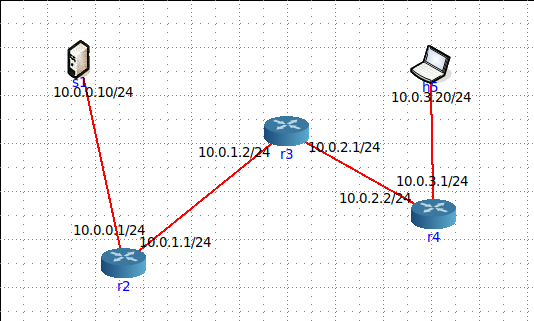
\includegraphics[width=\textwidth]{images/coreEx1.png}  
    \caption{Core}
    \label{fig:coreEx1}
\end{figure}

\subsection{Alínea a}
\textbf{Active o wireshark ou o tcpdump no pc s1. Numa shell de s1, execute o
comando traceroute -l para o endereço IP do host h5.}

\begin{figure}[H]
    \centering 
    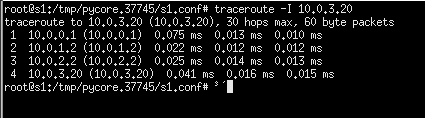
\includegraphics[width=\textwidth]{images/traceroutEx1.png}  
    \caption{Traceroute}
    \label{fig:traceroutEx1}
\end{figure}
\subsection{Alínea b}
\textbf{Registe e analise o tráfego ICMP enviado enviado por s1 e tráfego ICMP
recebido como resposta. Comente os resultados face ao comportamento esperado.}\\
Analisando os resultados obtidos, constatamos que o envio de pacotes teve duas
fases.\\
As fases estão divididas entre os pacotes com TTL abaixo de 4 e os com TTL acima
de 4.\\
Na primeira fase, os pacotes com TTL = 1, TTL = 2 e TTL = 3 foram descartados
pelos routers r1, r2 e r3, respetivamente. Para cada um destes foi recebido um
pacote \textit{Time-to-live exceeded}.\\
Na segunda fase, ao contrário dos pacotes anteriores, nenhum deles foi
descartado tendo como resposta pacotes \textit{Echo (ping) reply}.

\begin{figure}[H]
    \centering 
    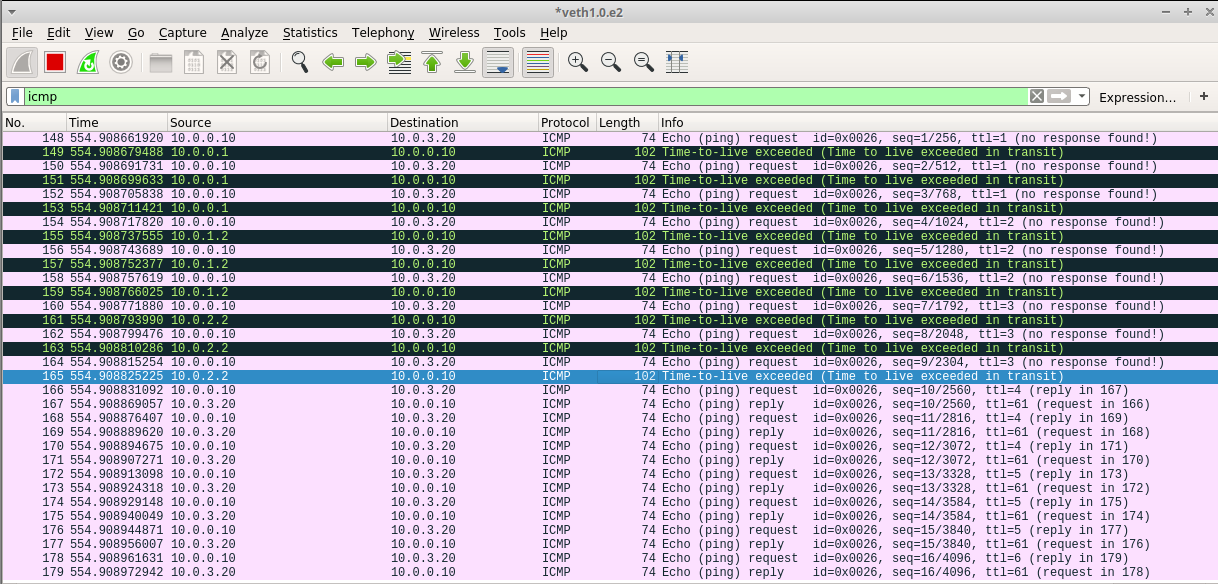
\includegraphics[width=\textwidth]{images/wiresharkEx1.png}  
    \caption{Wireshark}
    \label{fig:wiresharkEx1}
\end{figure}
\subsection{Alínea c}
\textbf{Qual deve ser o valor inicial mínimo do campo TTL para alcançar o
destino h5? Verifique na prática que a sua resposta está correta.}\\
Face aos resultados analisados na questão anterior, verifica-se que a partir de
TTL = 4 os pacotes deixam de receber mensagem de erro como resposta, logo o
valor inicial mínimo para alcançar o destino h5 será 4.

\subsection{Alínea d}
\textbf{Qual o valor médio do tempo de ida-e-volta (Round-Trip Time) obtido?}\\
O valor médio é obtido calculando a seguinte equação:
\begin{math}
RTT = ((0.075 + 0.013 + 0.010) / 3 + (0.022 + 0.012 + 0.012) / 3 + (0.025 +
0.014 + 0.013) / 3 + (0.041 + 0.016 + 0.015) / 3) * 2 = 0.178
\end{math}

\section{Exercício 2}

\begin{figure}[H]
    \centering 
    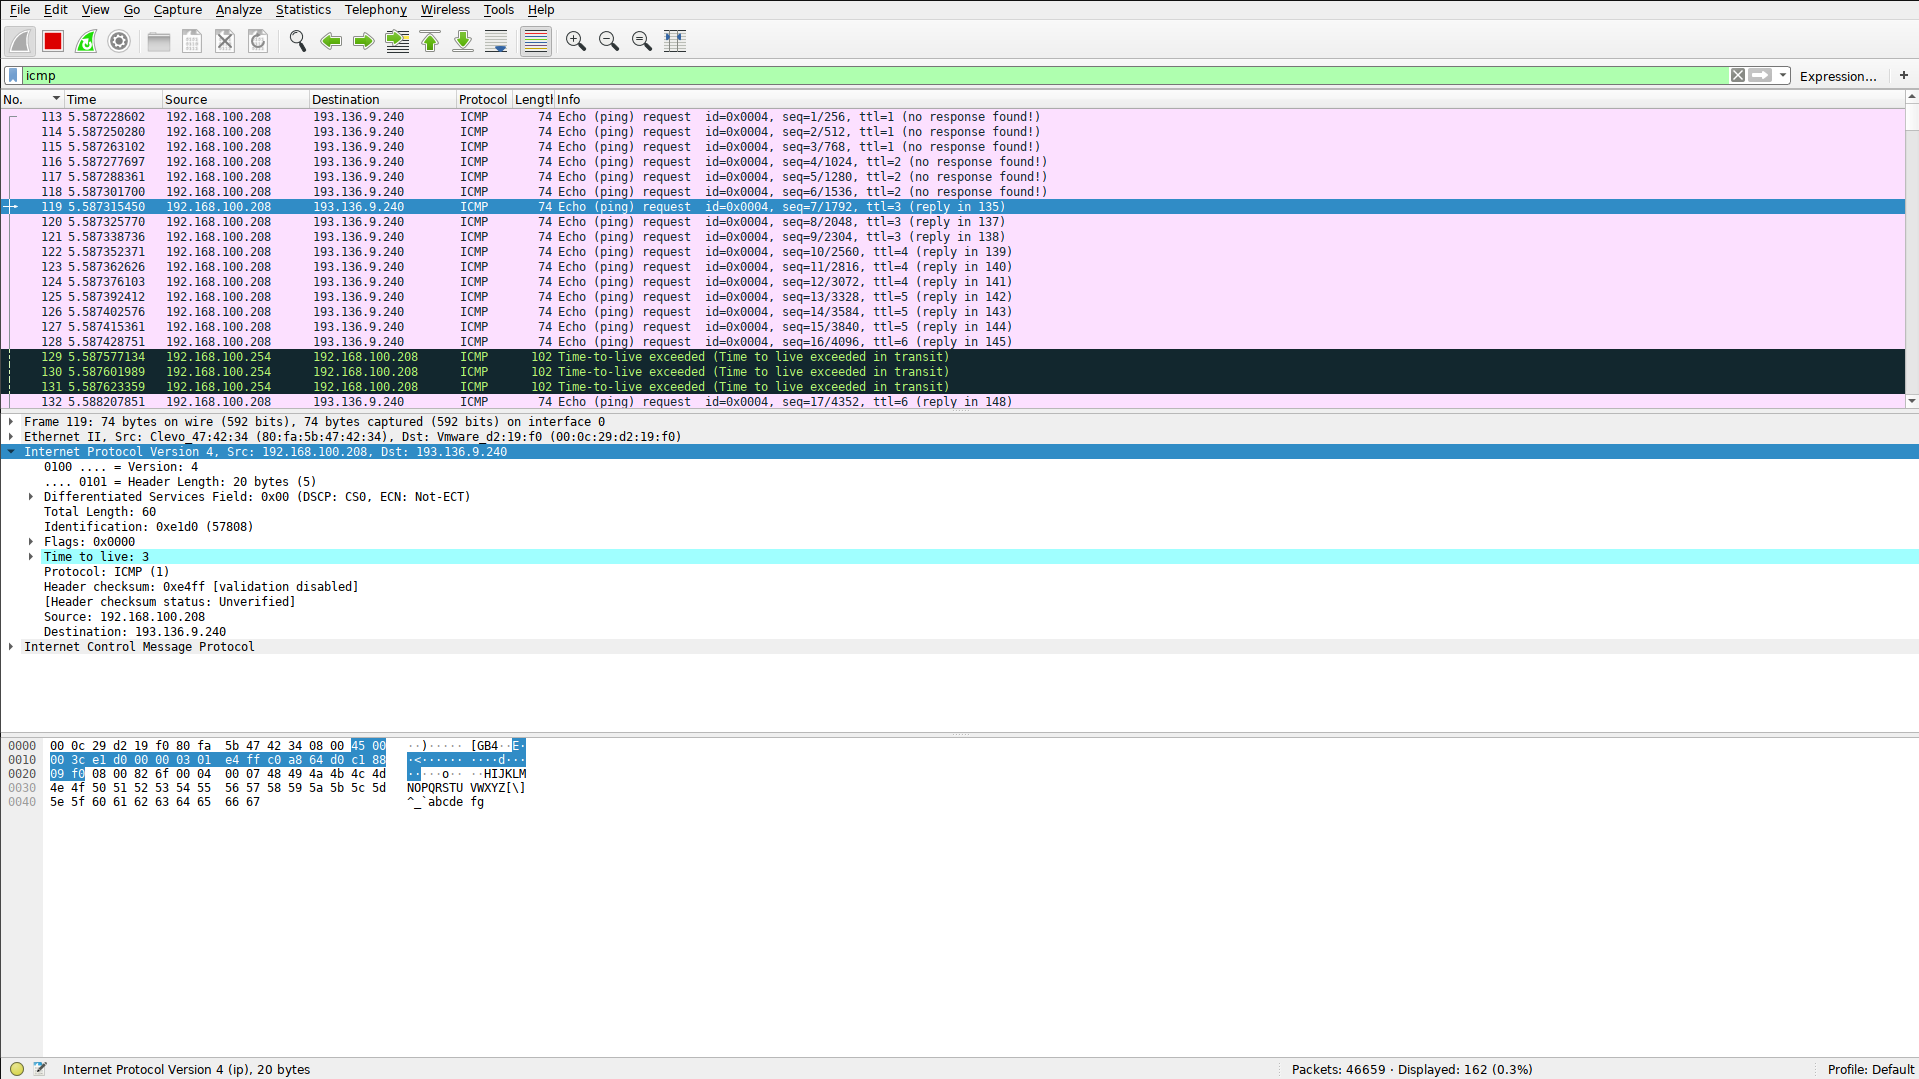
\includegraphics[width=\textwidth]{images/wiresharkEx2.png}  
    \caption{Wireshark}
    \label{fig:wiresharkEx2}
\end{figure}

\subsection{Alínea a}
\textbf{Qual é o endereço IP da interface ativa do seu computador?}
\begin{figure}[H]
    \centering 
    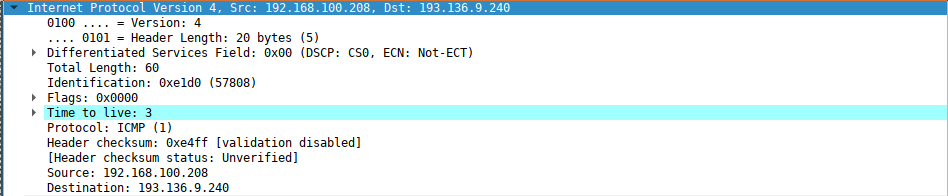
\includegraphics[width=\textwidth]{images/ipEx2.png}
    \caption{Cabeçalho IP}
    \label{fig:ipEx2}
\end{figure}
192.168.100.208

\subsection{Alínea b}
\textbf{Qual é o valor do campo protocolo? O que identifica?}\\
ICMP (1).\\
O valor do campo protocolo é 1, ou seja, identifica o protocolo ICMP.

\subsection{Alínea c}
\textbf{Quantos bytes tem o cabeçalho IP(v4)? Quantos bytes tem o campo de dados
(payload) do datagrama? Como se calcula o tamanho 
do payload?}\\
Analisando o campo Header length na figura \ref{fig:ipEx2}, conclui-se que o
cabeçalho IP tem 20 bytes.\\
O tamanho do campo de dados (\textit{payload}) é a diferença entre o número 
total de bytes e o tamanho do cabeçalho do datagrama. Logo, \textit{Payload} =
60 - 20 = 40 bytes.

\subsection{Alínea d}
\textbf{O datagrama IP foi fragmentado? }

\begin{figure}[H]
    \centering 
    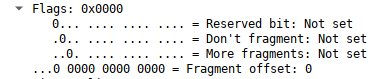
\includegraphics[width=\textwidth]{images/ipEx2Flags.png}
    \caption{Flags do Cabeçalho IP}
    \label{fig:ipEx2Flags}
\end{figure}
Observando a figura \ref{fig:ipEx2Flags} reparamos que no campo Flags, tudo está
a 0, logo o \textit{Fragment offset} tem valor 0, o que tendo em atenção agora a
flag \textit{More Fragments} concluímos que não existem mais fragmentos pois, se
o valor for 1 existem, caso contrário é 0. Logo, se estamos no primeiro
fragmento e não existem mais então este é o datagrama original.

\subsection{Alínea e}
\textbf{Ordene os pacotes capturados de acordo com o endereço IP fonte (e.g.,
selecionando o cabeçalho da coluna Source), e analise a sequência de tráfego
ICMP gerado a partir  do endereço IP atribuído à interface da sua máquina. Para
a sequência de mensagens ICMP enviadas pelo seu computador, indique que campos
do cabeçalho IP variam de pacote para pacote.}\\
Após ordenarmos, concluímos que os campos do cabeçalho IP que variam de pacote
para pacote são o \textit{TTL}, \textit{Header Checksum} e o identificador.

\begin{figure}[H]
    \centering 
    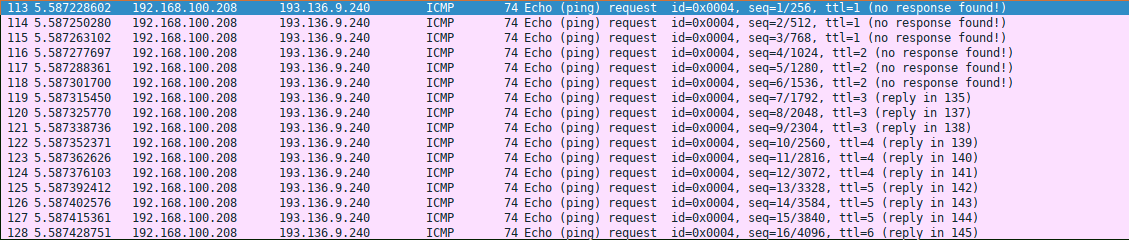
\includegraphics[width=\textwidth]{images/wiresharkSourceEx2.png}
    \caption{Tráfego Wireshark ordenado por endereço fonte}
    \label{fig:wiresharkSourceEx2}
\end{figure}
\subsection{Alínea f}
\textbf{Observa algum padrão nos valores do campo de Identificação do datagrama
IP e TTL?}\\
Ao analisar o datagrama IP, verificamos que este conserva os primeiros 8 bits em
todos o casos apresentados e os restantes são incrementados sequencialmente.\\
Também observamos que o TTL é incrementado sequencialmente

\subsection{Alínea g}
\textbf{Ordene o tráfego capturado por endereço destino e encontre a série de
repostas ICMP TTL exceeded enviadas ao seu computador. Qual é o valor do campo
TTL? Esse valor permanece constante para todas as mensagens de resposta ICMP TTL
exceed enviados ao seu host? Porquê?}\\
O valor do campo TTL é 62.\\
Para todas as mensagens de resposta \textit{ICMP TTL exceeded} recebidas no
nosso host esse valor manteve-se constante.\\
Apesar do TTL observado (pré-definido pelo destino) ser 64, quando o pacote chega ao
destino o TTL é de 62. Tal deve-se ao facto do pacote em questão ter passado por
2 routers antes de chegar e, por isso, ter sido decrementado 2 vezes.

\begin{figure}[H]
    \centering 
    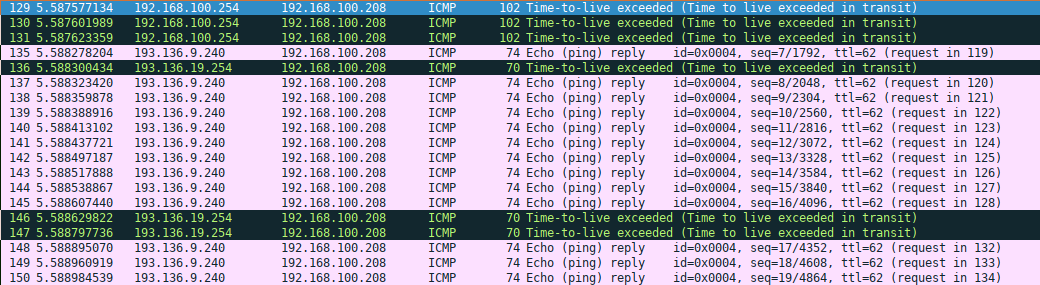
\includegraphics[width=\textwidth]{images/wiresharkDestinyEx2.png}
    \caption{Tráfego Wireshark ordenado por endereço de destino}
    \label{fig:wiresharkDestinyEx2}
\end{figure}

\section{Exercício 3}

\begin{figure}[H]
    \centering 
    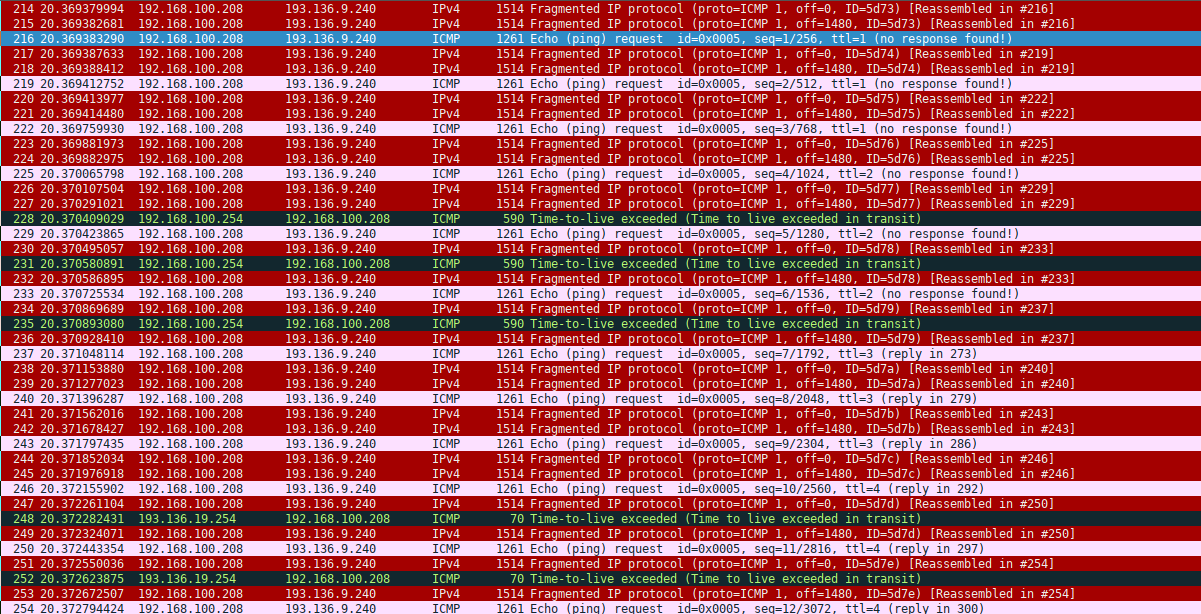
\includegraphics[width=\textwidth]{images/datagramaIpEx3.png}
    \caption{Fragmentos do datagrama IP}
    \label{fig:datagramaIpEx3}
\end{figure}
\subsection{Alínea a}
\textbf{Localize a primeira mensagem ICMP. Porque é que houve necessidade de
fragmentar o pacote inicial?}\\
Analisando a figura, vemos que a primeira mensagem ICMP é a 214.\\
Visto que o tamanho permitido pelo protocolo é inferior ao tamanho do PDU é
necessário que o pacote inicial seja fragmentado para poder circular na rede.

\subsection{Alínea b}
\textbf{Imprima o primeiro fragmento do datagrama IP segmentado. Que informação
no cabeçalho IP indica que se trata do primeiro fragmento? Qual é o tamanho
deste datagrama IP?}

\begin{figure}[H]
    \centering 
    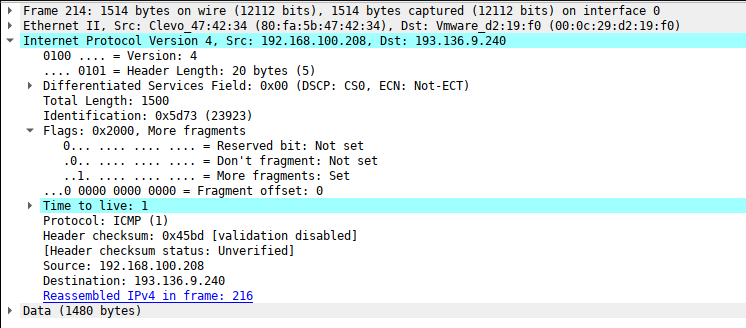
\includegraphics[width=\textwidth]{images/fragmentDatagramaIpEx3.png}
    \caption{Cabeçalho do primeiro fragmento do datagrama IP}
    \label{fig:fragmentDatagramaIpEx3}
\end{figure}
Podemos observar na figura que, no campo Flags, o \textit{More fragments} tem
valor 1, isso indica que o diagrama foi fragmentado, existindo então mais
fragmentos.\\
Seguidamente, podemos ver que o \textit{Fragment offset} é 0, provando de que se
trata do primeiro fragmento.\\
A \textit{Total Length} é igual a 1500 bytes.

\pagebreak
\subsection{Alínea c}
\textbf{Imprima o segundo fragmento do datagrama IP original. Que informação do
cabeçalho IP indica que não se trata do 1º fragmento? Há mais fragmentos? O que
nos permite afirmar isso?}

\begin{figure}[H]
    \centering 
    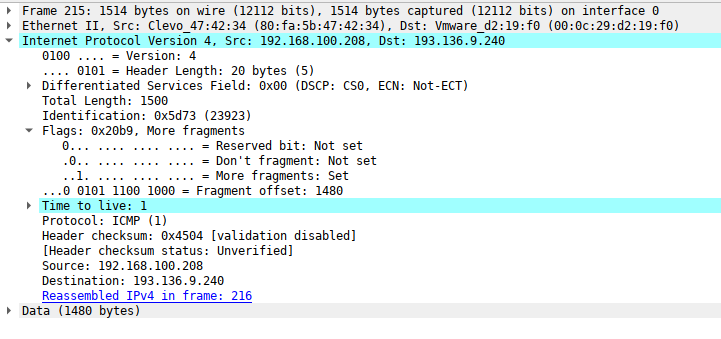
\includegraphics[width=\textwidth]{images/fragment2DatagramaIpEx3.png}
    \caption{Cabeçalho do segundo fragmento do datagrama IP}
    \label{fig:fragment2DatagramaIpEx3}
\end{figure}
Tal como já foi referido anteriormente, para se verificar se um fragmento é o
primeiro basta ter em atenção o valor que está no \textit{Fragment offset}. Se
esse valor for 0 então podemos concluir que se trata do primeiro. Como o valor
apresentado é diferente de 0 pudemos concluir que o fragmento em questão não se
trata do primeiro.\\
Podemos concluir que existem mais fragmentos pois o bit correspondente ao
\textbf{More fragments} é igual a 1.

\subsection{Alínea d}
\textbf{Quantos fragmentos foram criados a partir do datagrama original?
Como se detecta o último fragmento correspondente ao datagrama original?}\\
Como está mostrado na imagem, o terceiro fragmento do datagrama original
tem o bit correspondente a \textit{More fragments} a 0, ou seja, não há mais 
fragmentos a seguir a este. Concluindo assim que foram criados 3 fragmentos 
(214, 215 e 216).

\subsection{Alínea e}
\textbf{Indique, resumindo, os campos que mudam no cabeçalho IP entre os
diferentes fragmentos, e explique a forma como essa informação permite
reconstruir o datagrama original.}\\
Ao longo dos diferentes fragmentos, os campos do \textit{Fragment offset} e do
\textit{More Fragments} são alterados no cabeçalho IP.\\
O primeiro permite identificar a posição do fragmento no datagrama original. O
segundo indica se existem mais fragmentos do datagrama original para além do
próprio.


\chapter{Parte 2}

\section{Exercício 1}

\subsection{Alínea a}
\textbf{Indique que endereços IP e máscaras de rede foram atribuídos pelo CORE a
cada equipamento. Para simplificar, pode incluir uma imagem que ilustre de forma
clara a topologia definida e o endereçamento usado.}

\begin{figure}[H]
    \centering 
    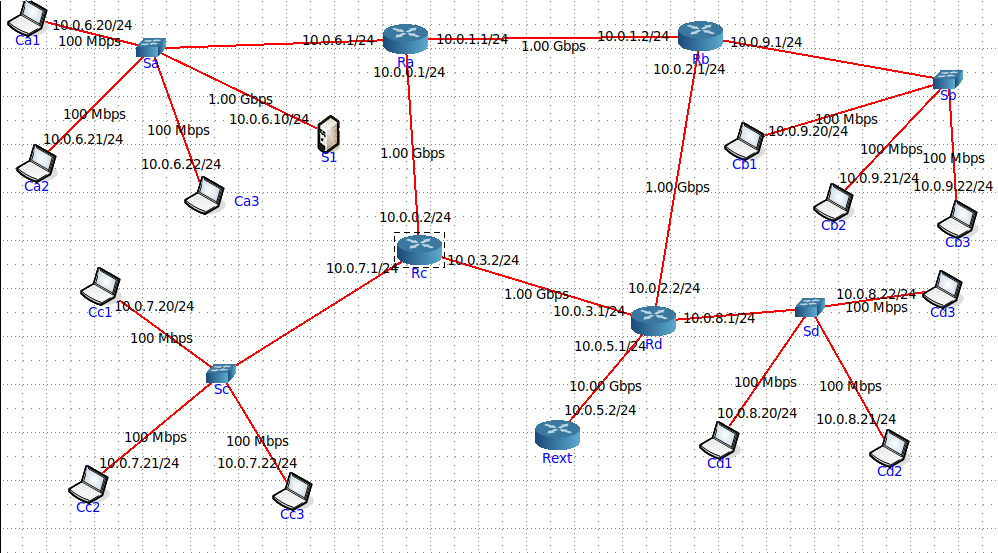
\includegraphics[width=\textwidth]{images/topologiaCore.png}
    \caption{Topologia Core}
    \label{fig:topologiaCore}
\end{figure}
Na figura \ref{fig:topologiaCore}, é possível verificar os endereços atribuídos
a cada equipamento. 

\subsection{Alínea b}
\textbf{Trata-se de endereços públicos ou privados? Porquê?}\\
Uma vez que todos os endereços utilizam um dos blocos reservados a endereços
privados: "10.0.0.0 - 10.255.255.255 / 8", concluimos que se tratam de endereços
privados.

\subsection{Alínea c}
\textbf{Por que razão não é atribuído um endereço IP aos switches?}\\
Não é necessário a atribuição de endereços IP aos switches porque são 
intervenientes na camade de ligação 2 e por sua vez transparentes à camada de
ligação 3. Estes encaminham os pacotes apenas tendo em atenção os endereços MAC
dos equipamentos.\\

\subsection{Alínea d}
\textbf{Usando o comando ping certifique-se que existe conectividade IP entre 
os laptops dos vários departamentos e o servidor do departamento A 
(basta certificar-se da conectividade de um laptop por departamento).}\\

\begin{figure}[H]
    \centering 
    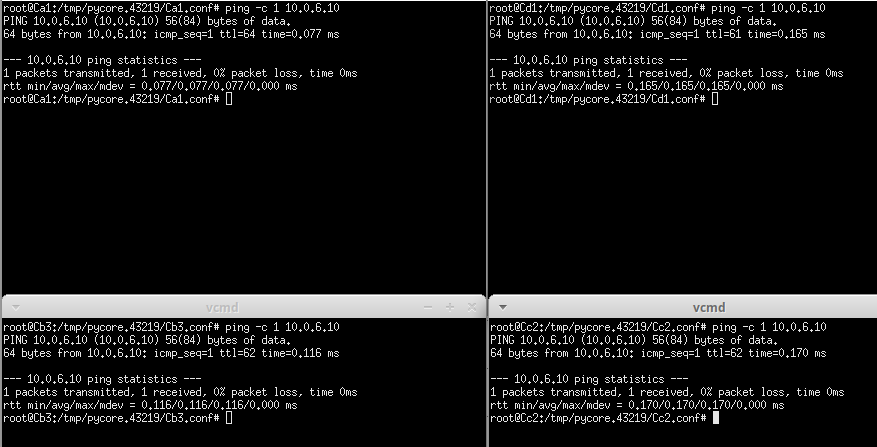
\includegraphics[width=\textwidth]{images/pingEx1P2.png}
    \caption{Conectividade entre os laptops de cada departamento e o servidor}
    \label{fig:pingEx1P2}
\end{figure}
Como podemos observar pela figura \ref{fig:pingEx1P2}, para verificar se existia
conectividade foi utilizado o comando ping em pelo menos um laptop de cada
departamento. Sendo que todos obtiveram resposta do servidor após terem enviado
pacotes, concluímos que existe conectividade em todos os departamentos.

\subsection{Alínea e}
\textbf{Verifique se existe conectividade IP do router de acesso Rext para o
servidor S1.}\\

\begin{figure}[H]
    \centering 
    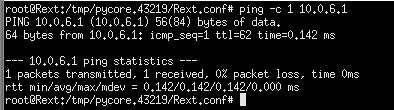
\includegraphics[width=\textwidth]{images/RextPing.png}
    \caption{Conectividade S1 - Router Rext}
    \label{fig:RextPing}
\end{figure}
Observando a figura \ref{fig:RextPing} e seguindo o racíocinio da alínea
anterior, verificamos que existe conectividade do router Rext para o servidor
S1.

\section{Exercício 2}

\subsection{Alínea a}
\textbf{Execute o comando netstat –rn por forma a poder consultar a tabela de
encaminhamento unicast (IPv4). Inclua no seu relatório as tabelas de
encaminhamento obtidas; interprete as várias entradas de cada tabela. Se
necessário, consulte o manual respetivo (man netstat).}

\begin{figure}[H]
    \centering 
    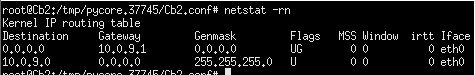
\includegraphics[width=\textwidth]{images/netstatPcEx2P2.png}
    \caption{Tabela de encaminhamento de um laptop do Departamento B}
    \label{fig:netstatPcEx2P2}
\end{figure}

\begin{figure}[H]
    \centering 
    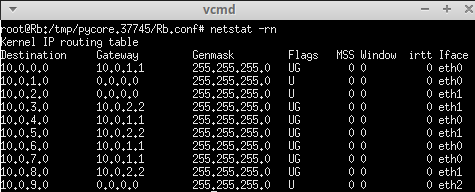
\includegraphics[width=\textwidth]{images/netstatRouterEx2P2.png}
    \caption{Tabela de encaminhamento do router Departamento B}
    \label{fig:netstatRouterEx2P2}
\end{figure}
Na figura \ref{fig:netstatPcEx2P2} está representada a tabela de encaminhamento
de onde podemos retirar informações relativa à rota que irá ser feita pelo
pacote. Na coluna "Destination" é nos indicado a sub-rede destino, na "Gateway"
a informação do equipamento pelo qual irá passar o pacote e na "Genmask" o tipo
da máscara.\\
Analisando a primeira e a segunda entrada da figura \ref{fig:netstatPcEx2P2} 
reparamos que as duas diferem no Gateway. Sendo que os dois endereços estão
ligados diretamente entre si, o Gateway não precisa de ser definido. Caso
contrário, seria necessário para se saber o próximo salto.\\
Relativamente à coluna Flags, estas apenas servem para acrescentar informações
adicionais. A flag "UG" é utilizada quando o gateway está definido e a "U" caso
contrário. Sendo que a primeira tabela e a segunda tabela são idênticas, não é
necessário fazer uma análise de todas as entradas da segunda.

\subsection{Alínea b}
\textbf{Diga, justificando, se está a ser usado encaminhamento estático ou
dinâmico (sugestão: analise que processos estão a correr em cada sistema).}

\begin{figure}[H]
    \centering 
    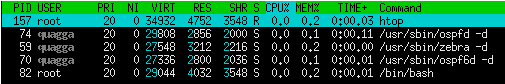
\includegraphics[width=\textwidth]{images/htop2a.png}
    \caption{Processos a serem executados em Ra}
    \label{fig:htop2a}
\end{figure}

\begin{figure}[H]
    \centering 
    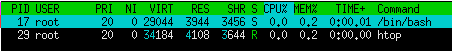
\includegraphics[width=\textwidth]{images/htopca1.png}
    \caption{Processos a serem executados em Ca1}
    \label{fig:htopca1}
\end{figure}
Se apenas analisassemos a figura \ref{fig:htop2a} reparavamos que é usado pelo router
o protocolo ospfd (este permite que o pacote siga diferentes caminhos quando um não é
possível) e assim concluiamos que se tratava de um encaminhamento dinâmico. No entanto,
após analisar a figura \ref{fig:htopca1} verificamos que não é usado esse protocolo,
conluindo então que se trata de um encaminhamento estático.

\subsection{Alínea c}
\textbf{Admita que, por questões administrativas, a rota por defeito (0.0.0.0 ou
default) deve ser retirada definitivamente da tabela de encaminhamento do
servidor S1 localizado no departamento A. Use o comando route delete para o
efeito. Que implicação tem esta medida para os utilizadores da empresa que
acedem ao servidor? Justifique.}

\begin{figure}[H]
    \centering 
    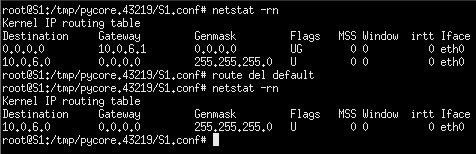
\includegraphics[width=\textwidth]{images/routeDelete.png}
    \caption{Remoção da rota default}
    \label{fig:routeDelete}
\end{figure}

\begin{figure}[H]
    \centering 
    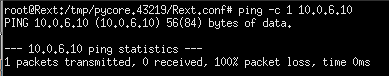
\includegraphics[width=\textwidth]{images/pingRextS1.png}
    \caption{Conectividade do Rext para S1}
    \label{fig:pingRextS1}
\end{figure}

\begin{figure}[H]
    \centering 
    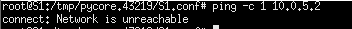
\includegraphics[width=\textwidth]{images/pingS1Rext.png}
    \caption{Conectividade do S1 para Rext}
    \label{fig:pingS1Rext}
\end{figure}

Removendo a rota por defeito é perdida a conectividade entre o servidor S1 e os 
restantes hosts existentes fora do departamento onde se encontra. Isto acontece porque o 
servidor S1 não tendo definida a rota de envio de tráfego para redes não locais faz com 
que não saiba para onde enviar de volta o que recebeu dos utilizadores. Tal verifica-se
nas figuras \ref{fig:pingRextS1} e \ref{fig:pingS1Rext} em que o router consegue enviar
para o servidor pacotes mas não os recebe de volta e este não consegue enviar
pacotes para o router.

\subsection{Alínea d}
\textbf{Adicione as rotas estáticas necessárias para restaurar a conectividade
para o servidor S1 por forma a contornar a restrição imposta na alínea c).
Utilize para o efeito o comando route add e registe os comandos que usou.}

\begin{figure}[H]
    \centering 
    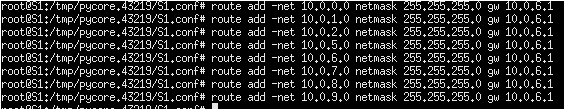
\includegraphics[width=\textwidth]{images/routeAdd.png}
    \caption{Restauração da conectividade adicionando rotas estáticas}
    \label{fig:routeAdd}
\end{figure}

\subsection{Alínea e}
\textbf{Teste a nova política de encaminhamento garantindo que o servidor está
novamente acessível utilizando para o efeito o comando ping. Registe a nova
tabela de encaminhamento do servidor.}

\begin{figure}[H]
    \centering 
    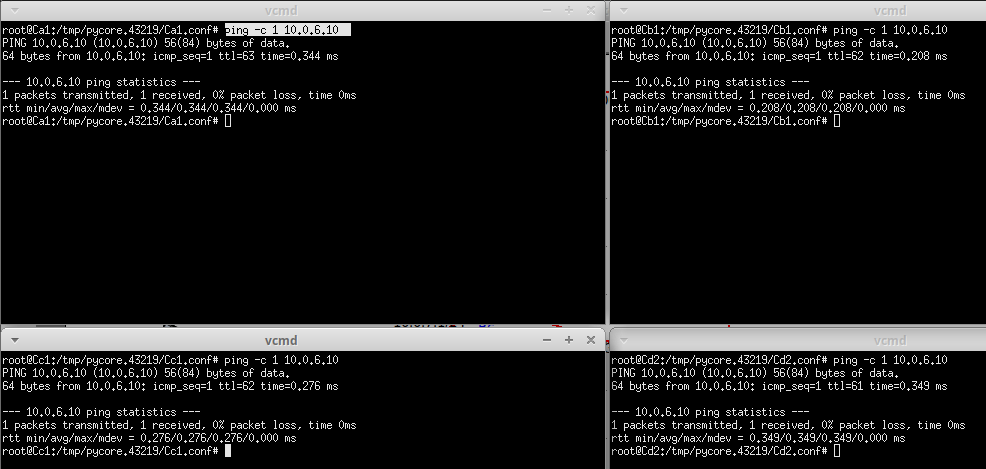
\includegraphics[width=\textwidth]{images/conectividadeDep.png}
    \caption{Conectividade entre os departamentos e S1}
    \label{fig:conectividadeDep}
\end{figure}

\begin{figure}[H]
    \centering 
    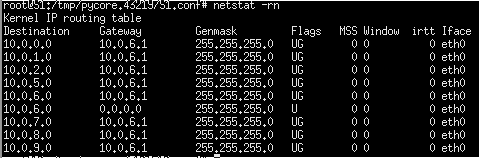
\includegraphics[width=\textwidth]{images/tabS1.png}
    \caption{Tabela de encaminhamento}
    \label{fig:tabS1}
\end{figure}

Analisando as figuras \ref{fig:conectividadeDep} e \ref{fig:tabS1} podemos verificar que
existe conectividade entre o servidor S1 e os laptops de todos os departamentos.

\section{Exercício 3}

\subsection{Alínea 1}

\textbf{Considere que dispõe apenas do endereço de rede IP 172.yyx.32.0/20, em
que “yy” são os dígitos correspondendo ao seu número de grupo (Gyy) e “x” é o
dígito correspondente ao seu turno prático (PLx). Defina um novo esquema de
endereçamento para as redes dos departamentos (mantendo a rede de acesso e core
inalteradas) e atribua endereços às interfaces dos vários sistemas envolvidos.
Deve justificar as opções usadas.}

\begin{figure}[H]
    \centering 
    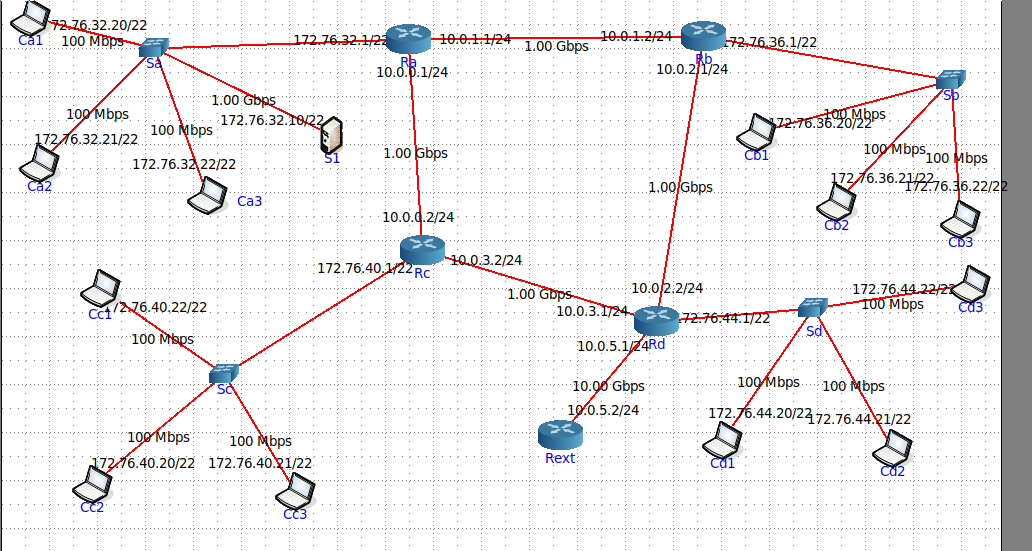
\includegraphics[width=\textwidth]{images/topCoreEx3.png}
    \caption{Topologia do novo endereçamento}
    \label{fig:topCoreEx3}
\end{figure}
O nosso grupo é o 7 e pertencemos ao PL6, logo o nosso endereço IP é 172.76.32.0/20.
Sendo que existem 4 departamentos então vão ser necessárias 4 sub-redes e
vai ser preciso usar 22 bits para suportar a topologia atual.
Assim, para cada departamento foram atribuídas as sub-redes:
\begin{itemize}
    \item Departamento A: 172.76.32.0/22
    \item Departamento B: 172.76.36.0/22
    \item Departamento C: 172.76.40.0/22
    \item Departamento D: 172.76.44.0/22
\end{itemize}


\subsection{Alínea 2}
\textbf{Qual a máscara de rede que usou (em notação decimal)? Quantos interfaces
IP pode interligar em cada departamento? Justifique.}\\
A máscara de rede que decidimos utilizar foi /22 o que corresponde a 255.255.252.0.
Como a máscara é /22 então temos 10 bits disponíveis para hosts, o que significa que 
temos $2^{10}$ - 2 hosts para cada departamento, ou seja, 1022 hosts.

\subsection{Alínea 3}
\textbf{Garanta e verifique que a conectividade IP entre as várias redes locais
da organização MIEI-RC é mantida. Explique como procedeu.}\\

\begin{figure}[H]
    \centering 
    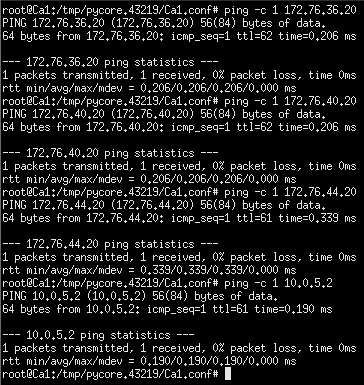
\includegraphics[width=0.5\textwidth]{images/pingEx3A.png}
    \caption{Conectividade a partir do Departamento A}
    \label{fig:pingEx3A}
\end{figure}

\begin{figure}[H]
    \centering 
    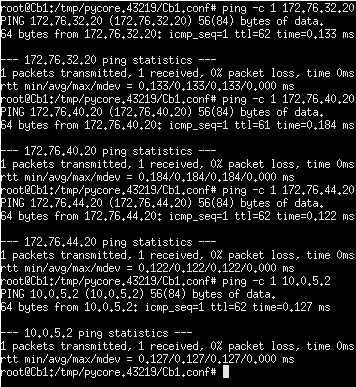
\includegraphics[width=0.5\textwidth]{images/pingEx3B.png}
    \caption{Conectividade a partir do Departamento B}
    \label{fig:pingEx3B}
\end{figure}

\begin{figure}[H]
    \centering 
    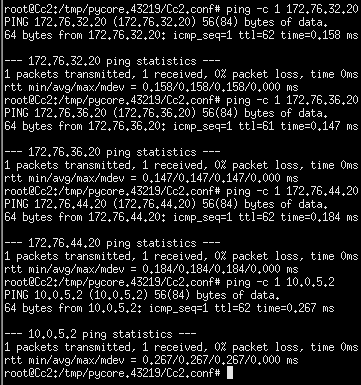
\includegraphics[width=0.5\textwidth]{images/pingEx3C.png}
    \caption{Conectividade a partir do Departamento C}
    \label{fig:pingEx3C}
\end{figure}

\begin{figure}[H]
    \centering 
    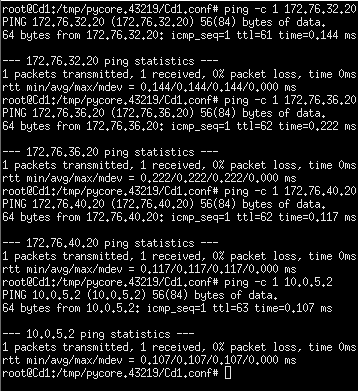
\includegraphics[width=0.5\textwidth]{images/pingEx3D.png}
    \caption{Conectividade a partir do Departamento D}
    \label{fig:pingEx3D}
\end{figure}
Analisando as figuras \ref{fig:pingEx3A}, \ref{fig:pingEx3B}, \ref{fig:pingEx3C} e
\ref{fig:pingEx3D} reparamos que existe conectividade entre todos os departamentos.

\chapter{Conclusão}
Neste trabalho prático foi nos dada a oportunidade de enriquecer o nosso conhecimento
relativamente a redes. Para isso foram usadas duas ferramentas: Core, para simulação de 
redes, e Wireshark, para captura de tráfego.\\
O trabalho está dividido em duas partes e cada uma delas dividida em 3 questões.
Cada parte teve como foco um tema e o mesmo acontece para cada questão facilitando a
nossa perceção em detalhes que mesmo não parecendo são relevantes.\\
Na primeira parte, o objetivo principal foi analisar o IP (Internet Protocol) e para isso
analisamos o formato dos pacotes/datagramas IP e fragmentação dos mesmos.\\
A segunda parte tinha como foco o estudo e perceção do endereçamento e encaminhamento do
que foi estudado na parte anterior. Construimos topologias na tentativa de simular 
o máximo do que se passa na realidade e nas mesmas remover, alterar e adicionar 
endereços para compreender como são feitos os transportes de pacotes numa rede.\\
Resumindo, consideramos que conseguimos atingir com sucesso todos os
desafios apresentados no enunciado obtendo assim um conhecimento mais avançado
sobre o protocolo IPv4 e \textit{sub-netting}.

\end{document}
